\documentclass[a4paper,12pt]{article}

\usepackage[utf8]{inputenc}
\usepackage{lmodern}
\usepackage[margin=1cm]{geometry}
\usepackage{amsmath}
\usepackage{graphicx}
\usepackage{xcolor}
\usepackage{caption}
\usepackage{tikz}
\usetikzlibrary{arrows.meta,positioning,shapes.geometric,calc,fit}

\pagestyle{empty}

\begin{document}
\begin{figure}[p]
  \centering
  \makebox[\textwidth][c]{\resizebox{1.08\textwidth}{!}{%
  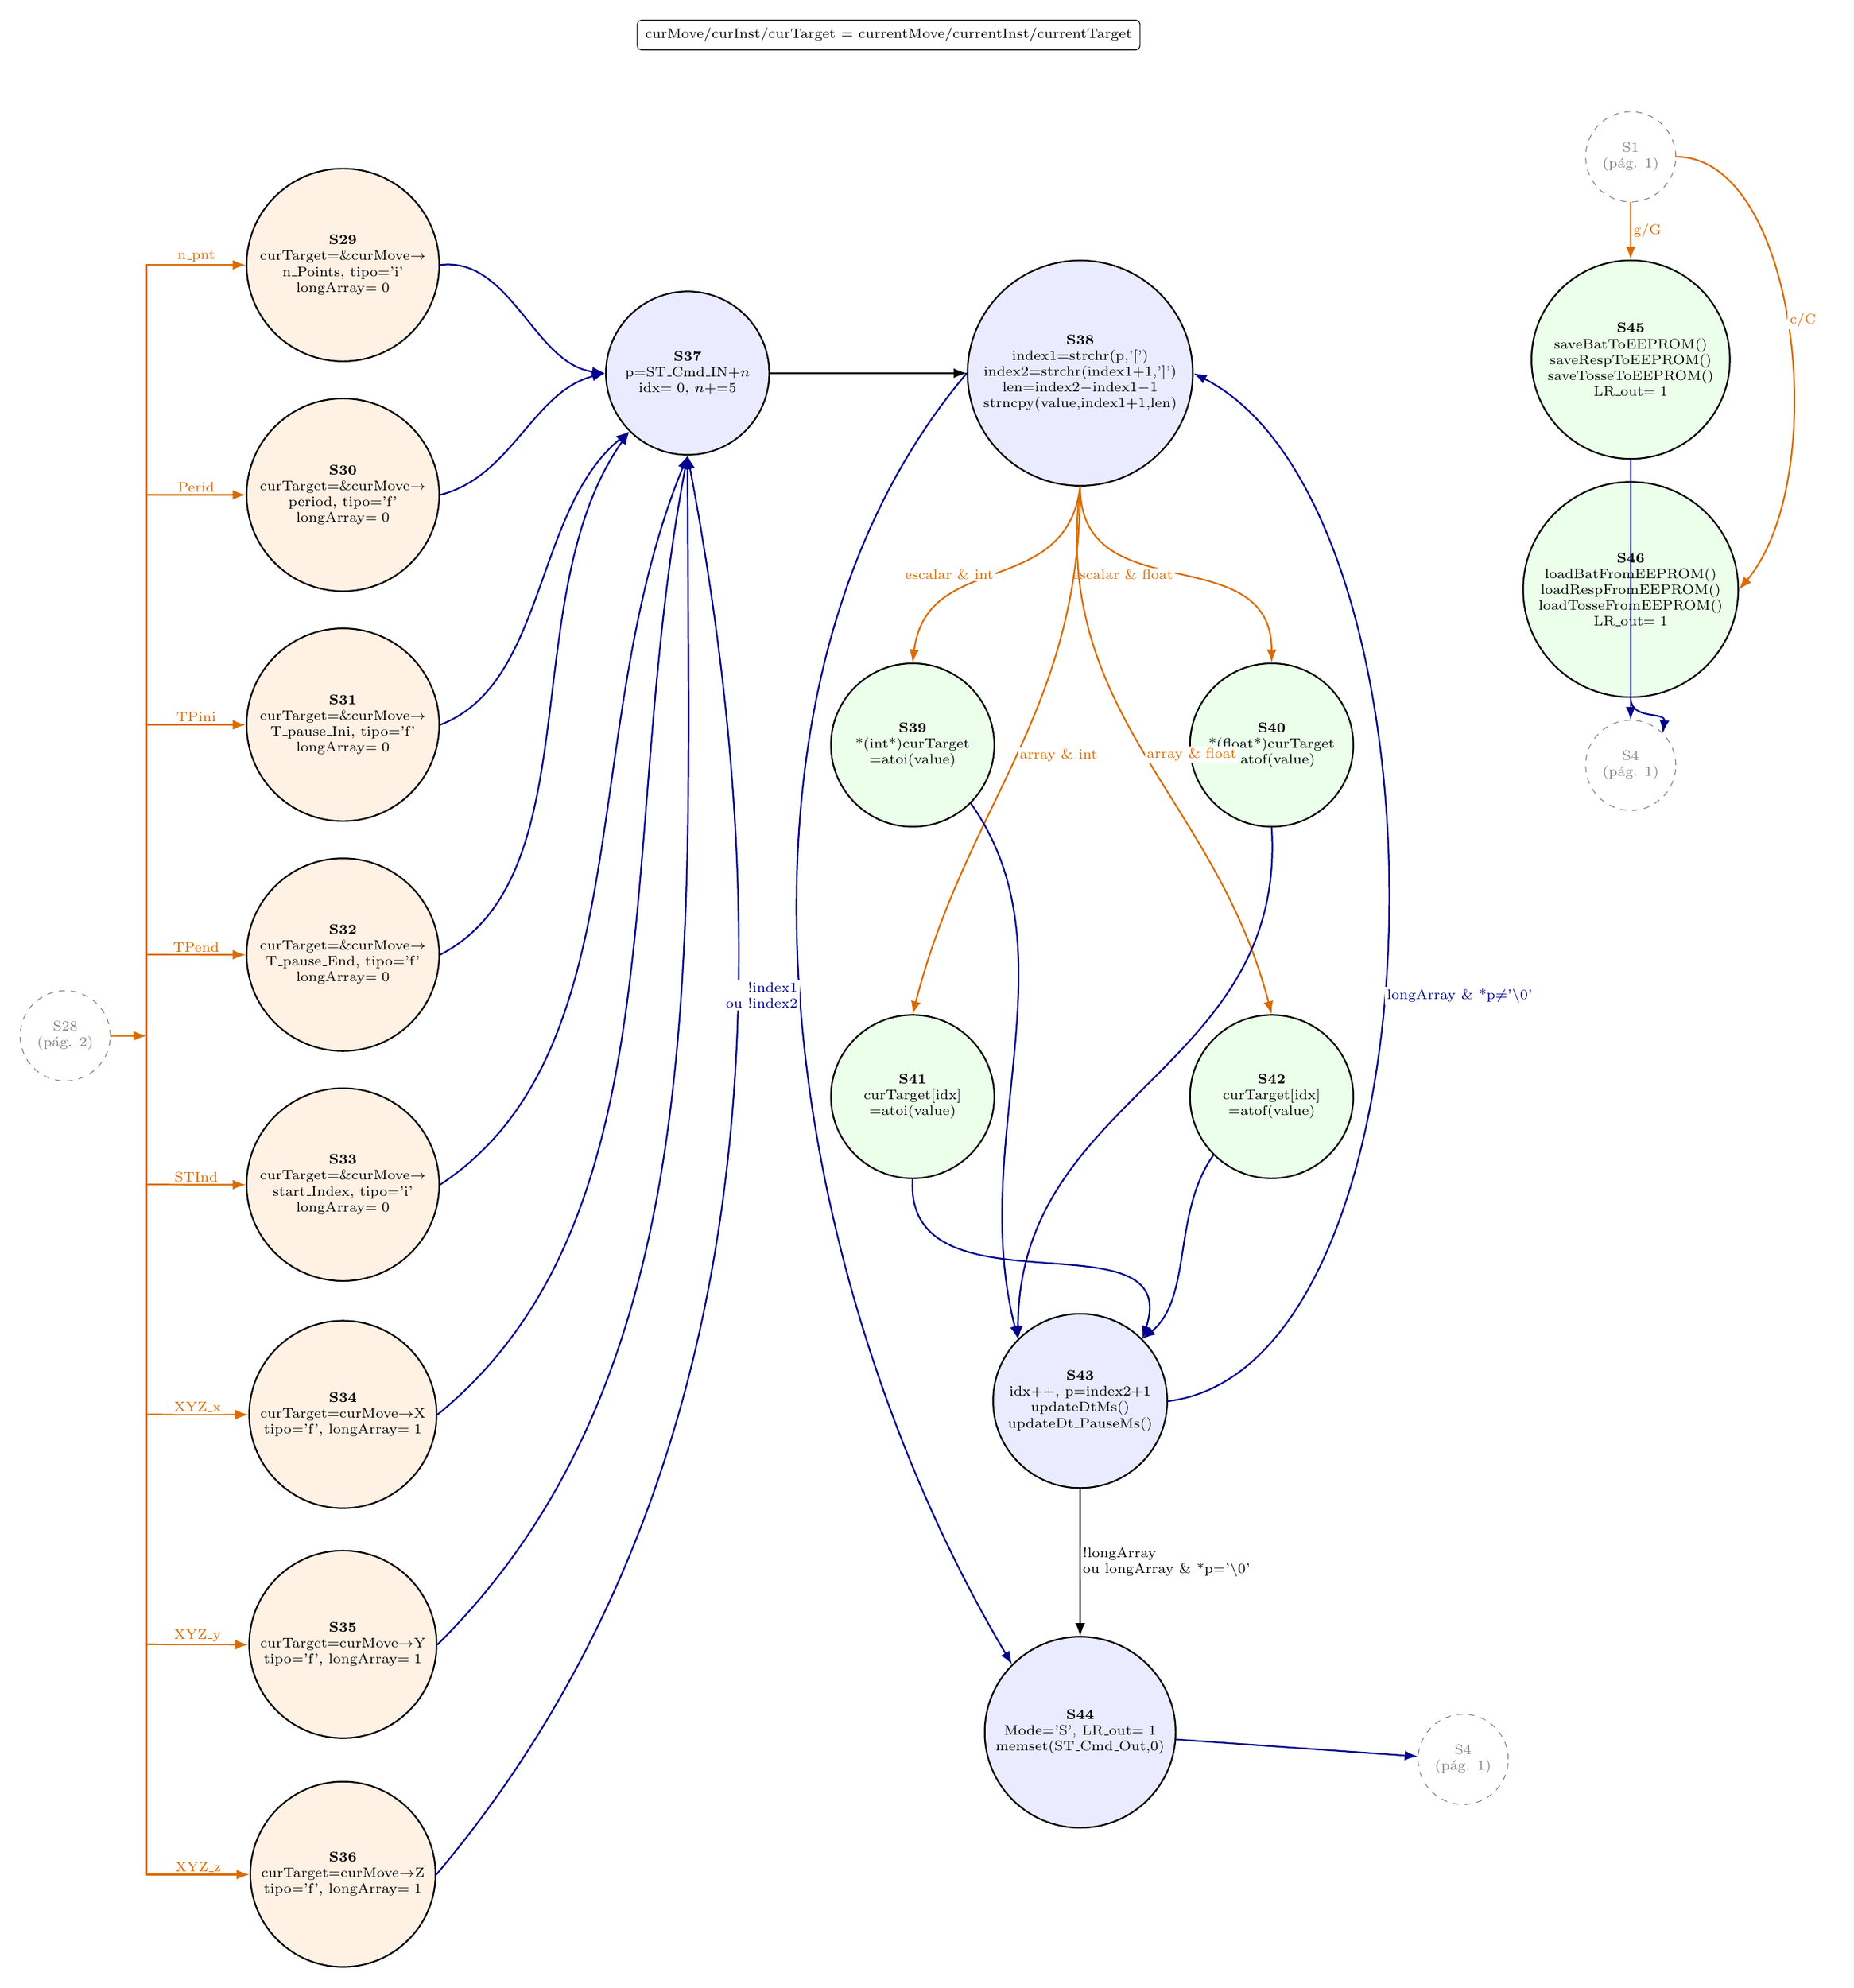
\begin{tikzpicture}[
    xscale=0.85, yscale=1.2,
    state/.style={draw, circle, align=center, minimum size=2.9cm, font=\scriptsize, thick},
    proxy/.style={draw, dashed, circle, align=center, minimum size=1.6cm, font=\scriptsize, gray},
    arrow/.style={-Latex, thick, line cap=round, line join=round},
    cmd/.style={-Latex, thick, orange!85!black, line cap=round, line join=round},
    ret/.style={-Latex, thick, blue!55!black, line cap=round, line join=round},
    lab/.style={font=\scriptsize, align=center, fill=white, inner sep=1pt},
    >=Stealth
  ]
    \node[draw, rounded corners=2pt, align=left, font=\scriptsize, fill=white, inner sep=4pt] at (0,2.2)
      {curMove/curInst/curTarget = currentMove/currentInst/currentTarget};

    \node[proxy] (p28) at (-17.2,-12.6) {S28\\(pág. 2)};

    \node[state, fill=orange!10] (c29) at (-11.4,-1.2) {\textbf{S29}\\curTarget$=$\&curMove$\to$\\n\_Points, tipo$=$'i'\\longArray$=0$};
    \node[state, fill=orange!10] (c30) at (-11.4,-4.6)  {\textbf{S30}\\curTarget$=$\&curMove$\to$\\period, tipo$=$'f'\\longArray$=0$};
    \node[state, fill=orange!10] (c31) at (-11.4,-8.0)  {\textbf{S31}\\curTarget$=$\&curMove$\to$\\T\_pause\_Ini, tipo$=$'f'\\longArray$=0$};
    \node[state, fill=orange!10] (c32) at (-11.4,-11.4)  {\textbf{S32}\\curTarget$=$\&curMove$\to$\\T\_pause\_End, tipo$=$'f'\\longArray$=0$};
    \node[state, fill=orange!10] (c33) at (-11.4,-14.8)   {\textbf{S33}\\curTarget$=$\&curMove$\to$\\start\_Index, tipo$=$'i'\\longArray$=0$};
    \node[state, fill=orange!10] (c34) at (-11.4,-18.2)   {\textbf{S34}\\curTarget$=$curMove$\to$X\\tipo$=$'f', longArray$=1$};
    \node[state, fill=orange!10] (c35) at (-11.4,-21.6)   {\textbf{S35}\\curTarget$=$curMove$\to$Y\\tipo$=$'f', longArray$=1$};
    \node[state, fill=orange!10] (c36) at (-11.4,-25.0)  {\textbf{S36}\\curTarget$=$curMove$\to$Z\\tipo$=$'f', longArray$=1$};

    \node[state, fill=blue!8] (c37) at (-4.2,-2.8)  {\textbf{S37}\\p$=$ST\_Cmd\_IN$+n$\\idx$=0$, $n{+}{=}5$};
    \node[state, fill=blue!8, minimum size=3.6cm] (c38) at (4.0,-2.8)  {\textbf{S38}\\index1$=$strchr(p,'[')\\index2$=$strchr(index1+1,']')\\len$=$index2$-$index1$-1$\\strncpy(value,index1+1,len)};

    \node[state, fill=green!8] (c39) at (0.5,-8.3) {\textbf{S39}\\*(int*)curTarget\\$=$atoi(value)};
    \node[state, fill=green!8] (c40) at (8.0,-8.3) {\textbf{S40}\\*(float*)curTarget\\$=$atof(value)};
    \node[state, fill=green!8] (c41) at (0.5,-13.5)  {\textbf{S41}\\curTarget[idx]\\$=$atoi(value)};
    \node[state, fill=green!8] (c42) at (8.0,-13.5)  {\textbf{S42}\\curTarget[idx]\\$=$atof(value)};

    \node[state, fill=blue!8] (c43) at (4.0,-18.0) {\textbf{S43}\\idx++, p$=$index2+1\\updateDtMs()\\updateDt\_PauseMs()};
    \node[state, fill=blue!8] (c44) at (4.0,-22.9) {\textbf{S44}\\Mode$=$'S', LR\_out$=1$\\memset(ST\_Cmd\_Out,0)};
    \node[proxy] (p4d) at (12.0,-23.3) {S4\\(pág. 1)};

    \node[proxy] (p1b) at (15.5,0.4)    {S1\\(pág. 1)};
    \node[state, fill=green!8] (c45) at (15.5,-2.6) {\textbf{S45}\\saveBatToEEPROM()\\saveRespToEEPROM()\\saveTosseToEEPROM()\\LR\_out$=1$};
    \node[state, fill=green!8] (c46) at (15.5,-6.0) {\textbf{S46}\\loadBatFromEEPROM()\\loadRespFromEEPROM()\\loadTosseFromEEPROM()\\LR\_out$=1$};
    \node[proxy] (p4e) at (15.5,-8.6) {S4\\(pág. 1)};

    \coordinate (cmdBusTop) at (-15.5,-1.2);
    \coordinate (cmdBusBot) at (-15.5,-25.0);
    \draw[thick, orange!85!black, line cap=round] (cmdBusTop) -- (cmdBusBot);
    \draw[cmd] (p28.east) -- (-15.5,-12.6);
    \draw[cmd] (cmdBusTop) -- node[lab, above]{n\_pnt} (c29.west);
    \draw[cmd] (-15.5,-4.6) -- node[lab, above]{Perid} (c30.west);
    \draw[cmd] (-15.5,-8.0) -- node[lab, above]{TPini} (c31.west);
    \draw[cmd] (-15.5,-11.4) -- node[lab, above]{TPend} (c32.west);
    \draw[cmd] (-15.5,-14.8) -- node[lab, above]{STInd} (c33.west);
    \draw[cmd] (-15.5,-18.2) -- node[lab, above]{XYZ\_x} (c34.west);
    \draw[cmd] (-15.5,-21.6) -- node[lab, above]{XYZ\_y} (c35.west);
    \draw[cmd] (cmdBusBot) -- node[lab, above]{XYZ\_z} (c36.west);

    \draw[ret] (c29.east) to[out=5,in=175] (c37.west);
    \draw[ret] (c30.east) to[out=10,in=190] (c37.west);
    \draw[ret] (c31.east) to[out=15,in=210] (c37.south west);
    \draw[ret] (c32.east) to[out=20,in=225] (c37.south west);
    \draw[ret] (c33.east) to[out=25,in=240] (c37.south);
    \draw[ret] (c34.east) to[out=30,in=255] (c37.south);
    \draw[ret] (c35.east) to[out=35,in=270] (c37.south);
    \draw[ret] (c36.east) to[out=40,in=285] (c37.south);

    \draw[arrow] (c37) -- (c38);
    \draw[cmd] (c38.south) to[out=-100,in=80] node[lab, left]{escalar \& int} (c39.north);
    \draw[cmd] (c38.south) to[out=-90,in=90] node[lab, left]{escalar \& float} (c40.north);
    \draw[cmd] (c38.south) to[out=-90,in=70] node[lab, right]{array \& int} (c41.north);
    \draw[cmd] (c38.south) to[out=-100,in=110] node[lab, right]{array \& float} (c42.north);
    \draw[ret] (c38.west) to[out=220, in=130, looseness=1] node[lab, left, align=right]{!index1\\ou !index2} (c44.north west);
    \draw[ret] (c39.south east) to[out=-45,in=110] (c43.north west);
    \draw[ret] (c40.south) to[out=-85,in=90] (c43.north west);
    \draw[ret] (c41.south) to[out=-95,in=65] (c43.north east);
    \draw[ret] (c42.south west) to[out=-135,in=30] (c43.north east);
    \draw[arrow] (c43) -- node[lab, right, align=left]{!longArray\\ou longArray \& *p$=$'\textbackslash 0'} (c44);
    \draw[ret] (c43.east) to[out=5,in=-20] node[lab, pos=0.45, right]{longArray \& *p$\neq$'\textbackslash 0'} (c38.east);
    \draw[ret] (c44) -- (p4d);

    \draw[cmd] (p1b) -- node[lab, right]{g/G} (c45);
    \draw[cmd] (p1b.east) to[out=0,in=40] node[lab, pos=0.48, right]{c/C} (c46.east);
    \draw[ret] (c45.south) to[out=-90,in=90] (p4e.north);
    \draw[ret] (c46.south) to[out=-90,in=80] (p4e.north east);
  \end{tikzpicture}}}
  \caption{FSM\_Serial\_Command (parte 3 de 3): seleção de campo, escrita do valor e comandos de EEPROM.}
  \label{fig:fsm-serial-command-p3}
\end{figure}

\end{document}
